
\lecture{Identidades Básicas}{lec03}


\section{Teoremas fundamentais}

\begin{frame}{Leis da álgebra booleana}

  \begin{description}
  \item<1-| alert@1>[Identidade] $A+0=A$ e $A\cdot{}0=0$
  \item<2-| alert@2>[Zero e Um] $A+1=1$ e $A\cdot{}0=0$
  \item<3-| alert@3>[Existência de complementos] $A+\overline{A}=1$ e
    $A\cdot{}\overline{A}=1$
  \item<4-| alert@4>[Comutativa] $A+B=B+A$ e $A\cdot{}B=B\cdot{}A$
  \item<5-| alert@5>[Associativa] $A+(B+C)=(A+B)+C$ e
    $A\cdot{}(B\cdot{}C)=(A\cdot{}B)\cdot{}C$
  \item<6-| alert@6>[Distributiva] $A\cdot{}(B+C)=(A\cdot{}B)+(A\cdot{}C)$ \\
    $A+(B\cdot{}C)=(A+B)\cdot{}(A+C)$
  \end{description}
  
\end{frame}

\section{Teoremas de Morgan}

 \begin{frame}{Teoremas de Morgan}
   
\begin{columns}
\begin{column}{.5\textwidth}   
\framesubtitle{Augustus De Morgan, 1806--1871}
   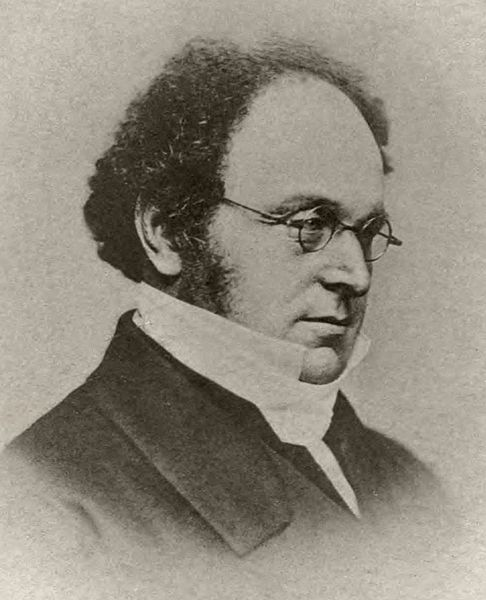
\includegraphics[scale=.15]{\imgdir/morgan.png}
\end{column}
\begin{column}{.5\textwidth}   
    $$\overline{A\cdot{}B} = \overline{A}+\overline{B}\eqno(1)$$
  $$\overline{A+{}B} = \overline{A}.\overline{B}\eqno(2)$$
\end{column}
\end{columns}

 \end{frame}
